% Font options: 10pm, 11pt, 12pt
% Align headings left instead of center: nocenter
\documentclass[xcolor=x11names,compress]{beamer}\usepackage[]{graphicx}\usepackage[]{color}
%% maxwidth is the original width if it is less than linewidth
%% otherwise use linewidth (to make sure the graphics do not exceed the margin)
\makeatletter
\def\maxwidth{ %
  \ifdim\Gin@nat@width>\linewidth
    \linewidth
  \else
    \Gin@nat@width
  \fi
}
\makeatother

\definecolor{fgcolor}{rgb}{0.345, 0.345, 0.345}
\newcommand{\hlnum}[1]{\textcolor[rgb]{0.686,0.059,0.569}{#1}}%
\newcommand{\hlstr}[1]{\textcolor[rgb]{0.192,0.494,0.8}{#1}}%
\newcommand{\hlcom}[1]{\textcolor[rgb]{0.678,0.584,0.686}{\textit{#1}}}%
\newcommand{\hlopt}[1]{\textcolor[rgb]{0,0,0}{#1}}%
\newcommand{\hlstd}[1]{\textcolor[rgb]{0.345,0.345,0.345}{#1}}%
\newcommand{\hlkwa}[1]{\textcolor[rgb]{0.161,0.373,0.58}{\textbf{#1}}}%
\newcommand{\hlkwb}[1]{\textcolor[rgb]{0.69,0.353,0.396}{#1}}%
\newcommand{\hlkwc}[1]{\textcolor[rgb]{0.333,0.667,0.333}{#1}}%
\newcommand{\hlkwd}[1]{\textcolor[rgb]{0.737,0.353,0.396}{\textbf{#1}}}%
\let\hlipl\hlkwb

\usepackage{framed}
\makeatletter
\newenvironment{kframe}{%
 \def\at@end@of@kframe{}%
 \ifinner\ifhmode%
  \def\at@end@of@kframe{\end{minipage}}%
  \begin{minipage}{\columnwidth}%
 \fi\fi%
 \def\FrameCommand##1{\hskip\@totalleftmargin \hskip-\fboxsep
 \colorbox{shadecolor}{##1}\hskip-\fboxsep
     % There is no \\@totalrightmargin, so:
     \hskip-\linewidth \hskip-\@totalleftmargin \hskip\columnwidth}%
 \MakeFramed {\advance\hsize-\width
   \@totalleftmargin\z@ \linewidth\hsize
   \@setminipage}}%
 {\par\unskip\endMakeFramed%
 \at@end@of@kframe}
\makeatother

\definecolor{shadecolor}{rgb}{.97, .97, .97}
\definecolor{messagecolor}{rgb}{0, 0, 0}
\definecolor{warningcolor}{rgb}{1, 0, 1}
\definecolor{errorcolor}{rgb}{1, 0, 0}
\newenvironment{knitrout}{}{} % an empty environment to be redefined in TeX

\usepackage{alltt}
%\documentclass[xcolor=x11names,compress,handout]{beamer}
\usepackage[]{graphicx}
\usepackage[]{color}
\usepackage{booktabs}
\usepackage{hyperref}
\usepackage{tikz}
\usepackage{multirow}
\usepackage{dcolumn}
\usepackage{bigstrut}
\usepackage{amsmath} 
\usepackage{xcolor,colortbl}
\usepackage{amssymb}
%\newcommand{\done}{\cellcolor{teal}#1}

%% Beamer Layout %%%%%%%%%%%%%%%%%%%%%%%%%%%%%%%%%%
\useoutertheme[subsection=false,shadow]{miniframes}
\useinnertheme{default}
\usefonttheme{serif}
\usepackage{Arev}
\usepackage{pdfpages}

\setbeamerfont{title like}{shape=\scshape}
\setbeamerfont{frametitle}{shape=\scshape, size=\normalsize}

\definecolor{dkblue}{RGB}{0,0,102}

\setbeamercolor*{lower separation line head}{bg=dkblue} 
\setbeamercolor*{normal text}{fg=black,bg=white} 
\setbeamercolor*{alerted text}{fg=red} 
\setbeamercolor*{example text}{fg=black} 
\setbeamercolor*{structure}{fg=black} 
 
\setbeamercolor*{palette tertiary}{fg=black,bg=black!10} 
\setbeamercolor*{palette quaternary}{fg=black,bg=black!10} 

\renewcommand{\(}{\begin{columns}}
\renewcommand{\)}{\end{columns}}
\newcommand{\<}[1]{\begin{column}{#1}}
\renewcommand{\>}{\end{column}}

\setbeamertemplate{navigation symbols}{} 
\setbeamertemplate{footline}[frame number]
\setbeamertemplate{caption}{\raggedright\insertcaption\par}

\setbeamersize{text margin left=5pt,text margin right=5pt}

%%%%%%%%%%%%%%%%%%%%%%%%%%%%%%%%%%%%%%%%%%%%%%%%%%




\title{Making Causal Critiques}
\subtitle{Day 3 - Assessing Causal Evidence}
\author{Jonathan Phillips}
\IfFileExists{upquote.sty}{\usepackage{upquote}}{}
\begin{document}

\frame{\titlepage}

\section{Introduction}

\begin{frame}
\frametitle{Solving the Problem of Causal Inference}
\begin{itemize}
\item We cannot!
\item But we can try and minimize the risks
\item Selecting units that provide appropriate counterfactuals, avoiding:
\begin{itemize}
\item Omitted variable bias
\item Selection Bias
\item Reverse Causation
\end{itemize}
\end{itemize}
\end{frame}

\begin{frame} 
\frametitle{Field Experiments}
\begin{itemize}
\item Field experiments provide confidence because treatment assignment is \textbf{controlled by the researcher}
\item But still take place in real-world environments, so they identify (hopefully) meaningful treatment effects
\end{itemize}
\end{frame}

\begin{frame}
\frametitle{Field Experiments}
\begin{itemize}
\item Why does randomization help us achieve causal inference?
\pause
\begin{itemize}
\item A treatment assignment mechanism that balances potential outcomes
\begin{itemize}
\item Every unit has \textbf{exactly the same} probability of treatment
\item No omitted variable bias
\item No self-selection
\item No reverse causation
\end{itemize}
\end{itemize}
\end{itemize}
\end{frame}

\begin{frame}
\frametitle{Field Experiments}
\begin{itemize}
\item Why does randomization help us achieve causal inference?
\begin{itemize}
\item We want to estimate:
\end{itemize}
\begin{eqnarray}
E(Y_1 - Y_0)
\end{eqnarray}
\pause
\begin{itemize}
\item Our data provides:
\end{itemize}
\begin{eqnarray}
E(Y_1|D=1)\text{ ,  }E(Y_0|D=0)
\end{eqnarray}
\pause
\begin{itemize}
\item With randomization, $Y_1, Y_0 \perp D$:
\end{itemize}
\begin{eqnarray}
E(Y_1|D=1) &=& E(Y_1) \\
E(Y_0|D=0) &=& E(Y_0) \\
E(Y_1|D=1) - E(Y_0|D=0) &=& E(Y_1) - E(Y_0) \\
&=& E(Y_1 - Y_0)
\end{eqnarray}
\end{itemize}
\end{frame}

\begin{frame}
\frametitle{Field Experiments}
\begin{itemize}
\item But these are just \textbf{expectations} (averages)
\pause
\begin{itemize}
\item On average, potential outcomes will be balanced
\item More likely in larger samples
\item We cannot verify potential outcomes
\item But we can assess balance in \textit{observable} covariates
\item What if some covariates are imbalanced? %Expected 1/20. Still need to correct as could be real bias.
\end{itemize}
\end{itemize}
\end{frame}

\begin{frame}
\frametitle{Field Experiments}
\begin{itemize}
\item Analysing field experiments
\begin{itemize}
\item Comparison of means: t-test to test significance
\item Regression achieves the same thing
\begin{itemize}
\item $Y_i \sim \alpha + \beta D_i + \epsilon_i$ 
\item $Y_i= Y_{0i} + (Y_{1i} - Y_{0i}) D_i + \epsilon_i$
\item Just the conditional expectation function: $E(Y|D=d)$
\end{itemize}
\item Include covariates if:
\begin{itemize}
\item There is residual imbalance
\item To increase precision of standard errors
\end{itemize}
\end{itemize}
\end{itemize}
\end{frame}

\begin{frame}
\frametitle{Field Experiments}
\begin{itemize}
\item Assumptions
\begin{itemize}
\item \textbf{Compliance with randomization} - Treatment was truly random and accepted
\item \textbf{SUTVA} - Treatment of one unit doesn't affect potential outcomes of other units
\item \textbf{Excludability} - Effects of treatment assignment operate \textbf{only} through treatment
\begin{itemize}
\item Depends if these effects are part of the causal chain
\end{itemize}
\end{itemize}
\end{itemize}
\end{frame}

\begin{frame}
\frametitle{Field Experiments}
\begin{itemize}
\item Limitations of Field Experiments: \textbf{Answerable Questions}
\pause
\begin{itemize}
\item Small sample sizes still prevent inference
\item Ethics
\item Logistics/Finance
\item Some treatments can't be manipulated (history)
\item Lack of control over treatment content and context - is it informative?
\item Long-term effects/adaptation?
\end{itemize}
\end{itemize}
\end{frame}

\begin{frame}
\frametitle{Field Experiments}
\begin{itemize}
\item Limitations of Field Experiments: \textbf{Internal Validity}
\pause
\begin{itemize}
\item No guarantee of actual balance (and Inefficient if we already know confounders)
\item Hawthorne effect: participants adapt behaviour in experiments
\item Biased measurement if not double-blind (non-excludability)
\item Average Treatment Effect can be skewed by Outliers
\item Always complications of non-compliance, SUTVA, attrition
\item Publication/Selection bias
\item Unbiased but imprecise; variation still high if lots of other variables also affect Y
\item Treatment assignment mechanism itself affects outcomes
\end{itemize}
\end{itemize}
\end{frame}

\begin{frame}
\frametitle{Field Experiments}
\begin{itemize}
\item All these complications mean we need lots of assumptions and background knowledge
\item Just as with other methodologies
\end{itemize}
\end{frame}

\begin{frame}
\frametitle{Lab Experiments}
\begin{itemize}
\item Causal Inference
\pause
\item Why lab experiments?
\pause
\begin{itemize}
\item Treatments we cannot administer in reality
\item Outcome measurements that are hard to take in reality
\item Random treatment assignment not permitted in reality
\end{itemize}
\end{itemize}
\end{frame}

\begin{frame}
\frametitle{Lab Experiments}
\begin{itemize}
\item \textbf{Treatment Assignment}: Same as a Field Experiment
\pause
\item \textbf{Treatment}: Not a manipulation of real world political or economic processes, but establishing controlled 'lab' conditions
\pause
\begin{itemize}
\item The advantage: Control over context helps isolate mechanisms
\item The disadvantage: Can we generalize to the real world from this artificial context?
\end{itemize}
\end{itemize}
\end{frame}

\begin{frame}
\frametitle{Natural Experiments}
\begin{itemize}
\item What is a natural experiment?
\pause
\begin{itemize}
\item Treatment assignment is independent of potential outcomes
\begin{itemize}
\item So randomized or 'as-if' random ('exogenous')
\end{itemize}
\pause
\item BUT The researcher doesn't control the treatment assignment process or treatment itself
\begin{itemize}
\item So not a field experiment
\end{itemize}
\item Can make possible analysis of questions that researchers might find unethical or impractical
\end{itemize}
\end{itemize}
\end{frame}

\begin{frame}
\frametitle{Natural Experiments}
\begin{table}[htbp]
  \centering
  \caption{Analysis Types and Assumptions}
    \resizebox*{1.1\textheight}{!}{\begin{tabular}{|r|l|p{2.5cm}|p{2.5cm}|p{2.5cm}|p{6cm}|}
    \hline
    \multicolumn{1}{|r|}{\textbf{Week}} & \multicolumn{1}{l|}{\textbf{Assumption:
}} & \textbf{Researcher Controls Treatment Assignment?} & \textbf{Treatment Assignment Independent of Potential Outcomes} & \textbf{SUTVA} & \multicolumn{1}{p{2cm}|}{\textbf{Additional Assumptions}} \bigstrut\\
    \hline
          & \textbf{Controlled Experiments} &       &       &       &  \bigstrut\\
    \hline
    1     &    Field Experiments & \checkmark & \checkmark & \checkmark &  \bigstrut\\
    \hline
    2     &    Survey and Lab Experiments &  \checkmark & \checkmark & \checkmark & Controlled Environment for treatment exposure \bigstrut\\
    \hline
          & \textbf{Natural Experiments} &       &       &       &  \bigstrut\\
    \hline
    3     &    Randomized Natural Experiments & X     & \checkmark & \checkmark &  \bigstrut\\
    \hline
    4     &    Instrumental Variables & X     & \checkmark & \checkmark & First stage and Exclusion Restriction (Instrument explains treatment but not outcome) \bigstrut\\
    \hline
    5     &    Regression Discontinuity & X     & \checkmark & \checkmark & Continuity of covariates; No manipulation; No compounding discontinuities \bigstrut\\
    \hline
          & \textbf{Observational Studies} &       &       &       &  \bigstrut\\
    \hline
    6     &    Difference-in-Differences & X     & X     & \checkmark & No Time-varying confounders; Parallel Trends \bigstrut\\
    \hline
    7     &    Controlling for Confounding & X     & X     & \checkmark & Blocking all Back-door paths \bigstrut\\
    \hline
    8     &    Matching & X     & X     & \checkmark & Overlap in sample characteristics \bigstrut\\
    \hline
    \end{tabular}}%
\end{table}%
\end{frame}

\begin{frame}
\frametitle{Natural Experiments}
\begin{itemize}
\item Three types of natural experiments
\begin{itemize}
\item 'Pure' natural experiments, where policy is as-if random
\item Instrumental Variables
\item Regression Discontinuities
\end{itemize}
\end{itemize}
\end{frame}

\begin{frame}
\frametitle{Natural Experiments}
\begin{itemize}
\item Because we don't control assignment, we need to verify the assumptions behind natural experiments
\begin{itemize}
\item How do we know assignment was truly random?
\item How was the treatment applied? Consistently?
\end{itemize}
\item We need 'Causal-process observations'
\end{itemize}
\end{frame}

\begin{frame}
\frametitle{Natural Experiments}
\begin{itemize}
\item Challenges due to lack of control over treatment:
\pause
\begin{itemize}
\item We must be lucky to 'find' natural experiments; what if the treatments/experiments that exist don't answer useful political economy questions?
\item The treatment and control groups produced by 'nature' may not produce treatment and control groups which differ in ways that represent a causal effect of interest (Sekhon and Titiunik 2012)
\item We also must be lucky to find a sample that is relevant and interesting - unlike a controlled trial we don't control the recipients either (eg. if we care about states, not municipalities, the audits are no use)
\end{itemize}
\end{itemize}
\end{frame}

\begin{frame}
\frametitle{Natural Experiments}
\begin{itemize}
\item Challenges due to lack of control over treatment: 
\begin{itemize}
\item Spillovers can be an issue - treatment units affect control units' potential outcomes (eg. women's quotas discourage women in non-reserved seats)
\item Generalizability a very open question; what causal process does the experiment really capture?
\item The treatment assignment of a natural experiment might have unique effects (excludability)
\end{itemize}
\end{itemize}
\end{frame}



\begin{frame}
\frametitle{Instrumental Variables}
\begin{itemize}
\item What can we do when the treatment assignment mechanism is not 'as-if' random?
\pause
\item Natural experiments focus on a specific \textbf{part} of treatment assignment that is 'as-if' random
\pause
\item An 'instrument' is a variable which assigns treatment in an 'as-if' random way
\pause
\begin{itemize}
\item Or at least in a way which is 'exogenous' - not related to confounders
\item Even if other confounding variables \textbf{also} affect treatment
\end{itemize}
\end{itemize}
\end{frame}

\begin{frame}
\frametitle{Instrumental Variables}
\begin{itemize}
\item We can use the instrument to isolate 'as-if' random variation in treatment, and use that to estimate the effect of treatment on the outcome
\pause
\item NOT the effect of the instrument on the outcome
\end{itemize}
\end{frame}

\begin{frame}
\frametitle{Instrumental Variables}
\begin{itemize}
\item Example Instruments:
\begin{itemize}
\item Rainfall for conflict 
\item Sex-composition for effect of third child
\item Distance from the coast for exposure to slave trade
\end{itemize}
\end{itemize}
\end{frame}

\begin{frame}
\frametitle{Instrumental Variables}
\begin{itemize}
\item Instrumental Variables Assumptions
\begin{itemize}
\item \textbf{Strong First Stage:} The Instrument must \textbf{affect} the treatment
\pause
\item We can test this with a simple regression: $Treatment \sim Instrument$
\pause
\item The instrument should be a significant predictor of treatment
\item Rule-of-thumb: $F-statistic > 10$
\end{itemize}
\end{itemize}
\end{frame}

\begin{frame}
\frametitle{Instrumental Variables}
\begin{itemize}
\item Instrumental Variables Assumptions:
\begin{itemize}
\item \textbf{Exclusion Restriction:} The Instrument \textbf{ONLY} affects the outcome through its effect on treatment, and not directly
\pause
\item Formally, $cov(Instrument,\text{errors in main regression Y }\sim D)=0$
\pause
\item \textbf{We cannot test or prove this assumption!}
\pause
\item Theory and qualitative evidence needed to argue that the instrument is not correlated with any other factors affecting the outcome
\item Sometimes, the exclusion restriction may be more credible if we include controls
\end{itemize}
\end{itemize}
\end{frame}

\begin{frame}
\frametitle{Instrumental Variables}
\begin{itemize}
\item Instrumental Variables Methodology:
\pause
\begin{enumerate}
\item Use an all-in-one package, eg. \textit{ivreg} in the \textit{AER} package
\begin{itemize}
\item Specify the formula: $Y ~ D | Instrument$
\pause
\end{itemize}
\item Conduct 2-Stage Least Squares: 
\pause
\begin{itemize}
\item Isolate the variation in treatment caused by the instrument: $D \sim Instrument$
\pause
\item Save the predicted values from this regression: $\hat{D} = D \sim Instrument$
\pause
\item Estimate how the predicted values affect the outcome: $Y \sim \hat{D}$
\pause
\item Interpret the coefficient on $\hat{D}$
\end{itemize}
\end{enumerate}
\end{itemize}
\end{frame}

\begin{frame}
\frametitle{Instrumental Variables}
\begin{itemize}
\item IV Interpretation:
\pause
\begin{itemize}
\item Your coefficient is a causal estimate ONLY for units that were actually treated \textbf{because of the instrument}
\pause
\item They don't tell us about the causal effect for other units that never responded to the instrument
\pause
\item We call our causal effect estimate a 'Local Average Treatment Effect' (LATE)
\item 'Local' to the units whose treatment status actually changed
\pause
\end{itemize}
\item Remember, those 'Local' units are not representative so we can't generalize
\end{itemize}
\end{frame}



\begin{frame}
\frametitle{Regression Discontinuities}
\begin{itemize}
\item Natural Experiments
\begin{itemize}
\item As always, we need some 'as-if' random variation in assignment to treatment to get plausible counterfactuals
\pause
\item Regression discontinuities take advantage of social rules that \textbf{treat similar people differently}
\pause
\item Specifically, similar people with slightly different 'scores' are assigned to treatment/control
\end{itemize}
\end{itemize}
\end{frame}

\begin{frame}
\frametitle{Regression Discontinuities}
\begin{center}
\includegraphics[scale=0.45]{Scale.png}
\end{center}
\end{frame}

\begin{frame}
\begin{itemize}
\item Regression Discontinuity
\begin{itemize}
\item Treatment assignment is 'as-if' random only \textbf{really close to the threshold}
\pause
\[
D_i=
\begin{cases}
1 & \text{if }x_i \geq \bar{x} \\
0 & \text{if }x_i < \bar{x}
\end{cases}
\]
\pause
\item For units just above and below the threshold:
\begin{itemize}
\item Their covariates are almost the same
\item Their potential outcomes are (on average) almost the same
\item They are plausible counterfactuals for each other
\end{itemize}
\pause
\item So we can compare them directly
\end{itemize}
\end{itemize}
\end{frame}

\begin{frame}
\begin{itemize}
\item Example thresholds:
\begin{itemize}
\item Exam cutoffs
\item Age cutoffs
\item Policy eligibility rules
\item Close elections
\item Adminsitrative boundaries
\end{itemize}
\end{itemize}
\end{frame}

\begin{frame}
\begin{itemize}
\item Regresssion Discontinuity Variables:
\begin{itemize}
\item \textbf{Running Variable, $x_i$:} The \textit{continuous} variable to which the threshold/cutoff is applied, eg. exam score
\pause
\item \textbf{Treatment, $D_i$:} Binary 0/1 depending on whether the running variable is above or below the threshold ($x_i>=\bar{x}$)
\pause
\item \textbf{Outcome, $Y_i$:} Any subsequent outcome you have measured
\end{itemize}
\end{itemize}
\end{frame}

\begin{frame}
\begin{itemize}
\item Regression Discontinuity Assumptions:
\begin{itemize}
\item Potential outcomes vary continuously (are independent of treatment) at the threshold
\pause
\item Units cannot precisely control their score and sort either side of the threshold
\pause
\item The threshold is not chosen strategically
\pause
\item No compound treatments
\end{itemize}
\end{itemize}
\end{frame}

\begin{frame}
\begin{itemize}
\item Thresholds more likely to be exogenous if:
\pause
\begin{itemize}
\item Units are not aware of the threshold
\pause
\item The threshold is decided after units make choices
\pause
\item The running variable is hard to manipulate precisely
\pause
\end{itemize}
\item We need qualitative evidence to support these assumptions
\end{itemize}
\end{frame}

\begin{frame}
\begin{itemize}
\item We can check for sorting with a density test
\item If units are bunched just above the threshold, this suggests manipulation
\end{itemize}

\begin{center}
\includegraphics[scale=2]{figure/Density-2.pdf}
\end{center}
\end{frame}

\begin{frame}
\begin{itemize}
\item Three Regression Discontinuity Methodologies:
\begin{enumerate}
\item \textbf{Difference-in-means:} Define a small window either side of the threshold and compare average outcomes in this window
\begin{itemize}
\item But can be biased since the correlation of the running variable with the outcome will be ignored
\pause
\end{itemize}
\item \textbf{'Parametric' regression discontinuity:} Uses all the data and estimates:
$$Y_i = \alpha + \beta_1 Running\_Variable_i + \beta_2 Treatment_i + \epsilon_i$$
\begin{itemize}
\item We just control for the 'smooth' variation in the running variable and estimate the 'jump' impact of treatment with a binary variable (dummy)
\item We may need to make the running variable non-linear
\pause
\end{itemize}
\item \textbf{Combined approach:} Focus on values close to the threshold, but use a (local) regression
\begin{itemize}
\item What bandwidth around the threshold do we use?
\end{itemize}
\end{enumerate}
\end{itemize}
\end{frame}


\begin{frame}
\frametitle{Raw Data}
\begin{center}
\begin{knitrout}
\definecolor{shadecolor}{rgb}{0.969, 0.969, 0.969}\color{fgcolor}
\includegraphics[width=\maxwidth]{figure/chart1-1} 

\end{knitrout}
\end{center}
\end{frame}

\begin{frame}
\frametitle{'Binned' Data}
\begin{center}
\begin{knitrout}
\definecolor{shadecolor}{rgb}{0.969, 0.969, 0.969}\color{fgcolor}
\includegraphics[width=\maxwidth]{figure/chart2-1} 

\end{knitrout}
\end{center}
\end{frame}

\begin{frame}
\frametitle{1. Difference-in-Means}
\begin{center}
\begin{knitrout}
\definecolor{shadecolor}{rgb}{0.969, 0.969, 0.969}\color{fgcolor}
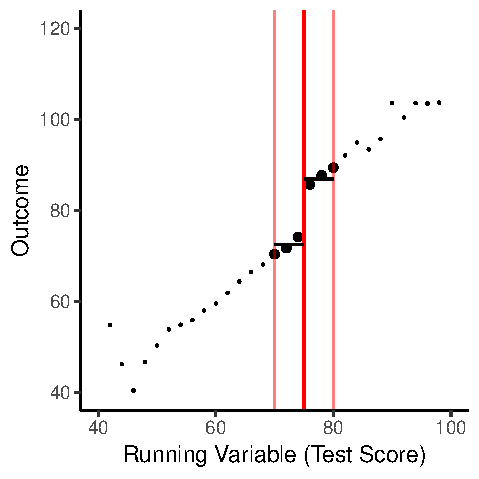
\includegraphics[width=\maxwidth]{figure/chart3-1} 

\end{knitrout}
\end{center}
\end{frame}

\begin{frame}
\frametitle{2a. Parametric Regression - Linear}
\begin{center}
\begin{knitrout}
\definecolor{shadecolor}{rgb}{0.969, 0.969, 0.969}\color{fgcolor}
\includegraphics[width=\maxwidth]{figure/chart4-1} 

\end{knitrout}
\end{center}
\end{frame}

\begin{frame}
\frametitle{2b. Parametric Regression - Non-linear}
\begin{center}
\begin{knitrout}
\definecolor{shadecolor}{rgb}{0.969, 0.969, 0.969}\color{fgcolor}
\includegraphics[width=\maxwidth]{figure/chart5-1} 

\end{knitrout}
\end{center}
\end{frame}

\begin{frame}
\frametitle{3. Combined Approach - Local Linear}
\begin{center}
\begin{knitrout}
\definecolor{shadecolor}{rgb}{0.969, 0.969, 0.969}\color{fgcolor}
\includegraphics[width=\maxwidth]{figure/chart6-1} 

\end{knitrout}
\end{center}
\end{frame}

\begin{frame}
\begin{itemize}
\item Which method?
\pause
\begin{itemize}
\item Difference-in-means is probably biased, and we can easily do better
\pause
\item The parametric approach uses more data (+precision) but depends on the right model: linear, quadratic, etc. (+risk of bias)
\pause
\item The combined approach uses less data (-precision) but is less dependent on the right model (-risk of bias)
\pause
\end{itemize}
\item In practice, apply all three as robustness checks
\end{itemize}
\end{frame}

\begin{frame}
\begin{itemize}
\item Why does RD estimate a \textbf{Local} Average Treatment Effect?
\pause
\begin{itemize}
\item Treatment assignment is only random at the threshold
\pause
\item Our estimates only apply to units close to the threshold
\pause
\item Units far from the threshold are very different for a reason, and causal effects are likely to be different
\end{itemize}
\end{itemize}
\end{frame}


\begin{frame}
\begin{itemize}
\item Limitations:
\begin{itemize}
\item Opportunistic regression discontinuities may not identify a useful causal effect or for a relevant group
\pause
\item Lots of alternative specifications so no single simple test
\pause
\item Less precise than a randomized trial, so we need more data
\pause
\item Risk of sorting/manipulation
\end{itemize}
\end{itemize}
\end{frame}

\begin{frame}
\begin{itemize}
\item Close elections are one type of regression discontinuity in which political office is 'as-if' randomized
\pause
\item Particularly useful for understanding the effects of political power
\pause
\begin{itemize}
\item \textbf{Running Variable: }Margin of victory
\item \textbf{Treatment: }Winning a close election
\item \textbf{Control: }Losing a close election
\item \textbf{Outcome: }Anything that happens later...
\end{itemize}
\end{itemize}
\end{frame}

\begin{frame}
\begin{itemize}
\item How much faith should we have in 'close election' regression discontinuities?
\pause
\item Eggers et al (2013):
\pause
\begin{itemize}
\item US House of Representatives elections show sorting in very close elections (<1\%)
\pause
\item Politicians (incumbents, the wealthy) can control whether they win, even when it's a tight race
\pause
\item They have extremely detailed information to predict vote results
\pause
\item So potential outcomes are not balanced
\pause
\item But no other case (9 countries) has this problem
\end{itemize}
\end{itemize}
\end{frame}




\begin{frame}
\frametitle{Difference-in-Differences}
\begin{itemize}
\item Our basic causal inference problem is that confounding makes counterfactual cases implausible (biased)
\pause
\item If we compare separate treatment and control units when treatment assignment is not random:
\begin{itemize}
\item The control units have different levels of the outcome for many reasons, not just treatment
\pause
\end{itemize}
\item If we compare the same unit before and after treatment:
\begin{itemize}
\item Other factors influencing the outcome might also have changed between our measurements (eg. any news event!)
\end{itemize}
\end{itemize}
\end{frame}

\begin{frame}
\frametitle{Difference-in-Differences}
\begin{itemize}
\item But what if we combine these approaches?
\pause
\item We can keep lots of variables fixed if we compare the same unit before and after treatment
\pause
\item We can measure how much other factors changed over time if we have units that were not exposed to treatment
\end{itemize}
\end{frame}

\begin{frame}
\frametitle{Difference-in-Differences}
\begin{itemize}
\item Example: How has Brexit affected the UK's growth rate?
\pause
\begin{itemize}
\item Comparing with European growth rates is biased - UK growth is influenced by oil, different labour laws etc.
\pause
\item Comparing before and after Brexit is biased - the world economy improved around the same time as Brexit (coincidentally)
\pause
\item But compare how European growth changes (-0.05\%) and UK growth changed (-0.4\%)
\pause
\item The net effect of Brexit is -0.35\%
\pause
\item That's two differences
\begin{itemize}
\item \textbf{Difference 1:} Between before and after (over time)
\item \textbf{Difference 2:} Between treated and control units
\pause
\end{itemize}
\end{itemize}
\end{itemize}
\end{frame}

\begin{frame}
\frametitle{Difference-in-Differences}
\begin{itemize}
\item We're now comparing \textit{changes} (differences), not \textit{levels} of the outcome
\begin{itemize}
\item Most confounders affect levels, so this makes our counterfactuals more plausible
\begin{itemize}
\item Eg. different laws affect growth rates, not the change in growth over time
\end{itemize}
\item And crucially, we can remove confounding even for \textit{unobserved} confounders
\item So Diff-in-Diff is 'better' than controlling or matching, which only eliminate observed (measured) confounding
\end{itemize}
\end{itemize}
\end{frame}

\begin{frame}
\frametitle{Difference-in-Differences}
\begin{itemize}
\item \textbf{BUT treatment assignment is still nowhere near random}
\pause
\item So this is not a natural experiment
\pause
\item Lots of confounders can still affect trends
\pause
\begin{itemize}
\item That creates bias in our causal estimates
\item Eg. the UK's growth rate was falling even before the Brexit vote, but Europe was improving
\pause
\end{itemize}
\item Diff-in-Diff is 'worse' than natural experiments
\end{itemize}
\end{frame}

\begin{frame}
\frametitle{Difference-in-Differences}
\begin{center}
\includegraphics[scale=0.3]{figure/UK_growth.png}
\end{center}
\end{frame}

\begin{frame}
\frametitle{Difference-in-Differences}
\begin{itemize}
\item Difference-in-differences only removes \textbf{time-invariant confounders}
\pause
\item Factors that create differences in the \textbf{levels} of the outcome variable for treatment and control units
\pause
\item We still need to \textbf{make the assumption and argument} that there are no time-varying confounders
\pause
\item Factors that affect the \textbf{trend} in the outcome \textit{differentially} in treated and control units
\pause
\item Eg. The UK had falling consumer confidence while confidence in the eurozone was improving
\end{itemize}
\end{frame}

\begin{frame}
\frametitle{Difference-in-Differences}
\begin{knitrout}
\definecolor{shadecolor}{rgb}{0.969, 0.969, 0.969}\color{fgcolor}
\includegraphics[width=\maxwidth]{figure/DinD_chart1-1} 

\end{knitrout}
\end{frame}


\begin{frame}
\frametitle{Difference-in-Differences}
\begin{knitrout}
\definecolor{shadecolor}{rgb}{0.969, 0.969, 0.969}\color{fgcolor}
\includegraphics[width=\maxwidth]{figure/DinD_chart1b-1} 

\end{knitrout}
\end{frame}

\begin{frame}
\frametitle{Difference-in-Differences}
\begin{knitrout}
\definecolor{shadecolor}{rgb}{0.969, 0.969, 0.969}\color{fgcolor}
\includegraphics[width=\maxwidth]{figure/DinD_chart1c-1} 

\end{knitrout}
\end{frame}

\begin{frame}
\frametitle{Difference-in-Differences}
\begin{itemize}
\item Estimating Difference-in-Differences
\pause
\item Time (Before and after) and treatment status (treated and control) are just variables in our data
\pause
\item We know how to do a regression for the effect of treatment status on the outcome
\end{itemize}
$$ Y_{it} = \alpha + \gamma D_i$$
\pause
\begin{itemize}
\item The difference-in-differences estimate is just the \textit{interaction} of time and treatment status
\end{itemize}
$$ Y_{it} = \alpha + \gamma D_i + \delta T_t + \beta D_i * T_t $$
\begin{itemize}
\item $\beta$ is our causal effect estimate
\end{itemize}
\end{frame}

\begin{frame}
\frametitle{Difference-in-Differences}
$$ Y_{it} = \alpha + \gamma D_i + \delta T_t + \beta D_i * T_t $$
\pause
\begin{itemize}
\item Difference-in-Differences means:
\end{itemize}
\small
$$ \big[ E(Y_{i,t=1}|D_i=1) - E(Y_{i,t=0}|D_i=1) \big] - \big[ E(Y_{i,t=1}|D_i=0) - E(Y_{i,t=0}|D_i=0) \big] $$
\normalsize
\end{frame}

\begin{frame}
\frametitle{Difference-in-Differences}
\small
$$ Y_{it} = \alpha + \gamma D_i + \delta T_t + \beta D_i * T_t $$
\pause
$$ E(Y_{i,t=1}|D_i=1) = \alpha + \gamma + \delta + \beta $$
\pause
$$ E(Y_{i,t=0}|D_i=1) = \alpha + \gamma $$
\pause
$$ E(Y_{i,t=1}|D_i=0) = \alpha + \delta $$
\pause
$$ E(Y_{i,t=0}|D_i=0) = \alpha $$
\pause
$$ \big[ E(Y_{i,t=1}|D_i=1) - E(Y_{i,t=0}|D_i=1) \big] = \delta + \beta $$
\pause
$$ \big[ E(Y_{i,t=1}|D_i=0) - E(Y_{i,t=0}|D_i=0) \big] = \delta $$
\pause
\footnotesize
$$ \big[ E(Y_{i,t=1}|D_i=1) - E(Y_{i,t=0}|D_i=1) \big] - \big[ E(Y_{i,t=1}|D_i=0) - E(Y_{i,t=0}|D_i=0) \big] = \beta $$
\normalsize
\end{frame}

\begin{frame}
\frametitle{Difference-in-Differences}
\begin{itemize}
\item The other way of thinking about the difference-in-differences estimator is as controlling for variation over time and between treated and control units
\pause
\item Including a variable for time is a fixed effect for time
\pause
\item Including a variable for treated/control is a fixed effect for treatment status
\pause
\item These 'remove' the 'levels' of variation between the treated and control units, and the 'overall trend' in all the data over time...
\pause
\item ...the only variation left in our data is the \textbf{differential} change over time between treated and control units
\pause
\item That's our causal effect
\end{itemize}
\end{frame}

\begin{frame}
\frametitle{Difference-in-Differences}
Raw Data:
\begin{knitrout}
\definecolor{shadecolor}{rgb}{0.969, 0.969, 0.969}\color{fgcolor}
\includegraphics[width=\maxwidth]{figure/DinD_chart2-1} 

\end{knitrout}
\end{frame}

\begin{frame}
\frametitle{Difference-in-Differences}
Add a variable (fixed effect) for treated/control:
\begin{knitrout}
\definecolor{shadecolor}{rgb}{0.969, 0.969, 0.969}\color{fgcolor}
\includegraphics[width=\maxwidth]{figure/DinD_chart3-1} 

\end{knitrout}
\end{frame}

\begin{frame}
\frametitle{Difference-in-Differences}
Add a variable (fixed effect) for time:
\begin{knitrout}
\definecolor{shadecolor}{rgb}{0.969, 0.969, 0.969}\color{fgcolor}
\includegraphics[width=\maxwidth]{figure/DinD_chart4-1} 

\end{knitrout}
\end{frame}

\begin{frame}
\frametitle{Difference-in-Differences}
Add a variable (fixed effect) for time:
\begin{knitrout}
\definecolor{shadecolor}{rgb}{0.969, 0.969, 0.969}\color{fgcolor}
\includegraphics[width=\maxwidth]{figure/DinD_chart5-1} 

\end{knitrout}
\end{frame}

\begin{frame}
\frametitle{Difference-in-Differences}
\begin{itemize}
\item How do we know if there are time-varying confounders?
\pause
\item We really want the outcome for the treated group to have the same trend as the control group
\pause
\begin{itemize}
\item So any difference in trend is only due to treatment
\pause
\end{itemize}
\item One test of this is to check if \textbf{pre-treatment trends are parallel}
\pause
\item Then our counterfactual makes sense
\end{itemize}
\end{frame}

\begin{frame}
\frametitle{Difference-in-Differences}
\begin{knitrout}
\definecolor{shadecolor}{rgb}{0.969, 0.969, 0.969}\color{fgcolor}
\includegraphics[width=\maxwidth]{figure/DinD_chart6-1} 

\end{knitrout}
\end{frame}

\begin{frame}
\frametitle{Difference-in-Differences}
\begin{knitrout}
\definecolor{shadecolor}{rgb}{0.969, 0.969, 0.969}\color{fgcolor}
\includegraphics[width=\maxwidth]{figure/DinD_chart7-1} 

\end{knitrout}
\end{frame}

\begin{frame}
\frametitle{Difference-in-Differences}
\begin{itemize}
\item Parallel trends (no time-varying confounders) is a difficult assumption
\item Selection into treatment is usually not just due to mostly 'fixed' variables (eg. gender) but due to 'time-varying' variables (eg. income, employment etc.)
\item Eg. training program participants' income has usually fallen a lot in the past few months
\pause
\item A good test is to see if there is an effect from 'placebos' - testing for treatment effects at times before treatment happened
\end{itemize}
\end{frame}

\begin{frame}
\frametitle{Difference-in-Differences}
\begin{itemize}
\item Even if pre-treatment trends are the same, treatment needs to be carefully defined:
\pause
\item Our estimate is based entirely on what affects treated units at a specific point in time
\pause
\item But many things may have changed at the same time
\pause
\item If these changes \textit{differentially} affect treated and control units, they change what we are estimating: a compound treatment
\pause
\item Eg. The UK also announced new rules to regulate the banking sector on the same day as Brexit
\end{itemize}
\end{frame}

\begin{frame}
\frametitle{Difference-in-Differences}
\begin{itemize}
\item Our groups need to be stable and unaffected by treatment
\item Eg. No migration due to treatment
\pause
\item Bertrand et al (2003):
\begin{itemize}
\item Careful with standard errors
\item Especially if more than two time periods (auto-correlation)
\item So cluster standard errors by each cross-sectional unit (eg. each country)
\end{itemize}
\end{itemize}
\end{frame}




\end{document}
 
 % effects of causes vs. reverse
